\chapter{Ecosystem definition}
\label{ecosystemDefinitionChapter}

The current and the following chapters define the ecosystem model used in the rest of the thesis. This chapter focuses on passive side of model, what builds an ecosystem, and relationships between these components. \autoref{simulationChapter} provides a dynamic description of the model and what happens to the ecosystem when the passage of time is taken into account.

\section{Agents}
Agents are heart of the ecosystem, they are components that can do something, interact with other components and change state of ecosystem. 

There are two types of agents - prey and predators. Predators hunt prey, which feeds on plants.

Each agent have two sets of parameters - features and needs. Features alters agent's abilities and efficiency and needs influence decision making.

\subsubsection{Species}
Only agents of the same species can breed with each other. There are two species present in ecosystem:
\begin{enumerate}
    \item Rabbit
    
    The rabbit is a representative of the prey. Rabbits eat carrots, drink water, reproduce with other rabbits and avoid the foxes that hunt them. They usually have about 6 offspring in a litter, but that number can vary depending on parents.
    
    \item Fox
    
    The fox is a predator. They do not eat plants, but hunt rabbits, which are their main and only source of food. Foxes reproduce more slowly than rabbits and their typical number of cubs is 4.
\end{enumerate}

A more detailed description of agents, including their features, needs, and how they make decisions can be found in \autoref{agentsChapter}

\begin{figure}
    \centering
    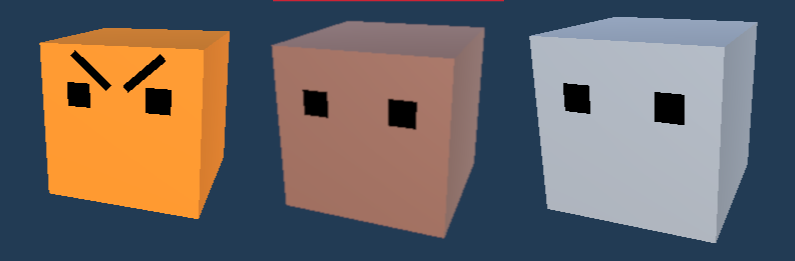
\includegraphics[width=\textwidth]{Images/agents.png}
    \caption{Graphical (GameObject) representation of agents used in Scene: fox, male rabbit and female rabbit.}
    \label{fig:agents}
\end{figure}

\section{Environment}
\subsection{Terrain}
The entire simulation takes place on a flat plane representing grass. There are two types of terrain in the environment - water and land. Agents cannot navigate through water, but they can satisfy their thirst near it. On land, individuals can move normally. 

\subsection{Food}
The environment contains food that is consumed by an herbivorous species. In this ecosystem there is only one species of plant - carrots. Carrots grow around certain points called \emph{Food Generators}. They appear at random points around the generator up to a certain number of plants, so new plants will only appear after the old ones have been eaten. 

The coordinates of a point $(x_f, y_f)$ in the Cartesian coordinate system relative to the generator position $(0, 0)$ are randomized and are represented by the following equation:

\begin{equation}
    x_f = r_f \cdot cos(\alpha)
\end{equation}
\begin{equation}
    y_f = r_f \cdot sin(\alpha)
\end{equation}
where
\begin{itemize}
    \item $r_f$ is random value in range $[0, r]$, $r$ is specific parameter defined in \hyperref[featuresNeedsStatesImplementation]{implementation}
    \item $\alpha$ is random angle in range $[0, 2\pi]$
\end{itemize}

Carrots grow over time, up to a certain maximum size. This is represented by growing in size. The longer a carrot lives, the larger it becomes and provides more energy to the individual who eats it. Carrots, unlike water, are consumed after being eaten by the rabbit, reducing its size. If the size is reduced below the minimum size, the carrot is considered to have been eaten whole and disappears from the ecosystem.

\begin{figure}
    \centering
    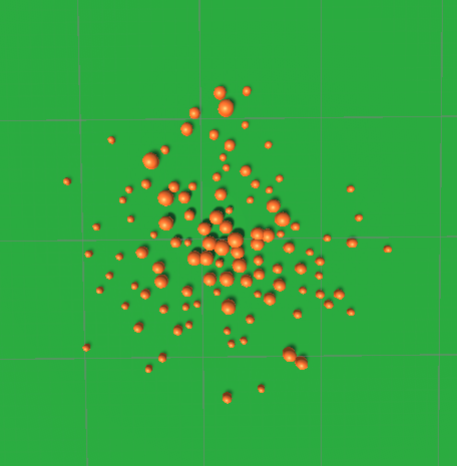
\includegraphics[width=\textwidth]{Images/carrot_generator_v2.png}
    \caption{Carrots around the generator with big maximum number of plants.}
    \label{fig:carrotGenerator}
\end{figure}

\subsection{Boundaries}
The ecosystem has specific dimensions. It is a square, with impassable barriers along its sides, beyond which agents cannot enter. Every element is located inside the boundaries.

\section{Interactions}
\label{interactionDescription}
Each interaction is initiated by an agent. There are two steps to initiate it. The agent must be ready to initiate the action, and then it must approach the object it wants to interact with. Interaction takes certain amount of time to complete and is different for each interaction, but interactions also can be instant. 

\subsubsection{Descriptions of each interaction}
Below you will find definitions of interactions between agents. A more detailed specification of these interactions, e.g. their duration, is included in \autoref{interactionsImplementationDescription}. A visual representation of interactions between agents can be found in \autoref{fig:interactionsDiagram}.
\begin{description}
    \item[Drinking] Happens between agents and water. Agent spend time near water satisfying thirst and at the end of interaction it reduces thirst by an amount proportional to the time spent drinking.
    \item[Mating] Happens between agents of the same species. Male agent need to find female partner that is willing to reproduce. If found partner do not have enough reproduction urge each interaction initiated by male agent will increase urge of its partner up to a point that mating can occur. New offspring are spawned at the end of interaction and new set of features is established through a genetic algorithm process. For more information, see \autoref{geneticAlgorithmsChapter}
    \item[Eating Carrot] Happens between rabbit and carrot. Similar to drinking agent spend some time near carrot and then reduces hunger by eaten amount. Here however carrot are consumed after interaction.
    \item[Eating Rabbit] Happens between fox and rabbit. Fox must find a rabbit and then eats it whole to reduce its hunger. Fox feeds one rabbit fully, reducing its hunger to zero.
\end{description}

\begin{figure}
    \centering
    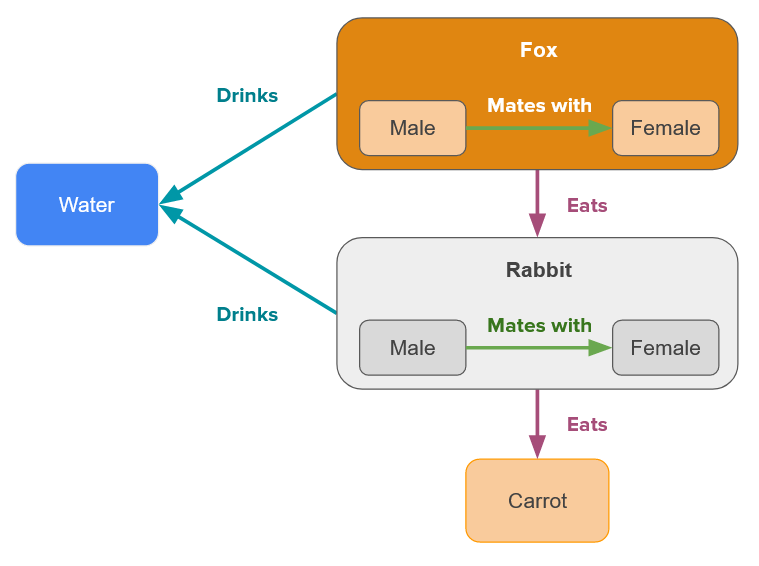
\includegraphics[width=\textwidth]{Images/interaction_diagram_v2.png}
    \caption{Diagram of interactions.}
    \label{fig:interactionsDiagram}
\end{figure}
